\documentclass[conference]{IEEEtran}
\usepackage{amsmath,amssymb}
\usepackage{graphicx}
\usepackage{booktabs}
\usepackage{listings}
\usepackage{url}
\usepackage{cite}
\usepackage{tikz}
\usetikzlibrary{shapes.geometric,arrows.meta,positioning,fit,backgrounds}

\begin{document}

\title{Fault-Tolerant Runtime Parsing for the Intent Marker Protocol: \\
Bounded Recovery and Layer-Wise Ablation}

\author{
\IEEEauthorblockN{Amihere Theophilus Junior}
\IEEEauthorblockA{Department of Computer Science and Engineering\\
University of Mines and Technology (UMaT)\\
Tarkwa, Ghana\\
amiheretheophilusjunior@gmail.com}
\and
\IEEEauthorblockN{Ezekiel Mensah Martey}
\IEEEauthorblockA{Department of Computer Science and Engineering\\
University of Mines and Technology (UMaT)\\
Tarkwa, Ghana\\
emmartey@umat.edu.gh}
\and
\IEEEauthorblockN{Dome Masselineous Gyielzaw}
\IEEEauthorblockA{Department of Computer Science and Engineering\\
University of Mines and Technology (UMaT)\\
Tarkwa, Ghana\\
Masskojo1@gmail.com}
\and
\IEEEauthorblockN{Ansong Maame Afia Dwamena}
\IEEEauthorblockA{Department of Computer Science and Engineering\\
University of Mines and Technology (UMaT)\\
Tarkwa, Ghana\\
maameansong36@gmail.com}
}

\maketitle

\begin{abstract}
Prior work evaluated the Intent Marker Protocol (IMP) against JSON-schema
function calling across Qwen-3-32B, Llama-3.3-70B, and gpt-oss-120b,
establishing compatibility for those tested models and token-scaling behavior
without independently isolating the downstream parser \cite{irai2026}. This
paper examines that parser independently. We present a five-layer
runtime architecture for tolerant intent-marker parsing -- protocol
facade, stream delimiter scanner, dual-dialect tolerant lexer,
compiler-bound schema unflattening, and incremental state synthesis --
and situate each layer against its nearest architectural precedent:
error-tolerant and incremental parsing, indentation-sensitive lexical
grammars, and static-metadata-driven schema mapping. We characterize
parser behavior against six classes of malformed intent-stream patterns and
report a cumulative ablation isolating the scanner, tolerant lexer, and compiler-bound
unflattening contributions. Across 750 deterministic recoverable cases, the
full system achieved 100.00\% exact syntactic recovery, compared with
76.00\% without compiler-bound unflattening, while preserving identical
final ASTs under monolithic and one-character stream delivery. We further
compare recovery behavior against an existing JSON-repair library and
quantify an under-reported failure mode: tolerant parsing without duplicate
detection can silently accept conflicting fields. The full
system rejected all 150 ambiguity controls.
\end{abstract}

\begin{IEEEkeywords}
Intent Marker Protocol, Fault-Tolerant Parsing, Error-Tolerant Compilation, Structured Output, Agentic LLMs, Incremental Parsing, Streaming Parsers
\end{IEEEkeywords}

\section{Introduction}

The Intent Marker Protocol (IMP) was introduced as an alternative to
provider-native JSON function calling, separating tool communication
(a compact DSL) from output validation (a downstream parser), and was
shown empirically across Qwen-3-32B, Llama-3.3-70B, and gpt-oss-120b to
avoid the observed provider-level exclusions, reduce schema-declaration token overhead by 47\%,
and reduce aggregate effective input tokens by 6.32$\times$ at 100 registered
tools \cite{irai2026}. That evaluation measured end-to-end protocol behavior
but did not independently perturb or ablate the downstream parser. In
practice, LLM output streams are not always
well-formed -- payloads truncate mid-generation, network transport
fragments delimiters across packet boundaries, and models emit
semi-structured text that violates strict JSON grammar. \cite{irai2026}
explicitly identifies comparison against generation-layer constrained
decoding as ``the most important open technical question for journal
follow-up.'' Before that comparison can be interpreted, the downstream parser's
own contribution must be separated from model behavior. This paper provides
that mechanism-level ablation and grounds each architectural decision against
existing parsing and schema-mapping literature.

This paper makes the following contributions:
\begin{enumerate}
\item A five-layer runtime architecture for tolerant intent-marker
parsing, each layer motivated by and contrasted against an established
architectural lineage (error-tolerant compilation, incremental parsing,
indentation-sensitive grammars, static schema mapping).
\item A compiler-bound schema unflattening layer that resolves flat or
aliased LLM output through explicitly authorized compiler paths, coupled to
a bounded ambiguity and execution policy.
\item A characterization of six distinct malformed-stream failure
patterns and the recovery mechanism for each.
\item A cumulative layer-wise ablation on a 900-case suite, including 150
ambiguity controls, with a separate 4,000-trial transport-fragmentation sweep.
\item An over-tolerance analysis of configurations that silently accept
conflicting fields rather than rejecting ambiguity, a correctness risk
under-reported in tolerant-parsing evaluations.
\end{enumerate}

Accordingly, the evaluation asks three mechanism-level questions: how much
recovery is contributed by the scanner, lexer, and schema integration; whether
final ASTs are invariant to transport chunking; and whether ambiguous inputs
are rejected rather than silently coerced. It does not attempt to rank IMP
against generation-layer constrained decoding on end-to-end accuracy or latency.

\section{Background and Related Work}

\subsection{Structured Output Generation Paradigms}

Existing approaches to constraining LLM output into structured form fall
into three paradigms, summarized in Table~\ref{tab:taxonomy}.
\textbf{Constrained decoding} (XGrammar \cite{xgrammar}, SGLang
\cite{sglang}, Outlines \cite{outlines}) restricts generation according to
a formal grammar or schema during decoding, preventing output outside the
accepted grammar when generation completes successfully under the supported
constraint. This requires generation-time control of token selection and
introduces grammar-processing or token-filtering overhead.
\textbf{Provider-native protocols} (OpenAI function calling, Gemini function
declarations) instead expose vendor-managed structured-generation interfaces;
their internal enforcement mechanisms are implementation-specific, and model
or schema availability can vary \cite{irai2026}.
\textbf{Application-layer downstream tolerant parsing}, the subject of this paper,
decouples generation from validation entirely: the model streams plain
text or IMP markers, and a client-side parser tolerantly reconstructs
structured output without constraining generation or requiring a provider's
structured-output interface.

\begin{table}[t]
\centering
\caption{Structured-output design space. The approaches prevent or handle
malformation at different pipeline stages and are not interchangeable.}
\label{tab:taxonomy}
\scriptsize
\resizebox{\columnwidth}{!}{%
\begin{tabular}{@{}llll@{}}
\toprule
Approach & Control locus & Partial state & Malformation policy \\
\midrule
Constrained decoding & Generation-time decoder & Decoder-specific & Prevent out-of-grammar syntax \\
Provider-native & Vendor service & Provider-specific & Provider-managed \\
Downstream IMP & Client runtime & Yes & Bounded recovery \\
\bottomrule
\end{tabular}}
\end{table}

\subsection{Error-Tolerant and Incremental Parsing}

Classical compiler recovery continues past syntax violations by locally
resynchronizing on recognizable tokens \cite{burkefisher}; incremental parsers
maintain partial trees while input arrives \cite{wagnergraham,treesitter}.
Layers 2 and 3 adapt these ideas to structurally plausible LLM completions,
using IMP delimiters rather than statement boundaries as resynchronization
points. Unlike tree-sitter's optimization for re-parsing after editor changes,
the scanner targets zero-leakage buffering under arbitrary network chunking, a
transport-specific failure mode.

\subsection{Indentation-Sensitive and Tolerant Lexical Grammars}

YAML \cite{yamlspec} demonstrates whitespace-delimited structure, while JSON5
\cite{json5spec} relaxes JSON quoting and comma rules. Layer 3's contribution
is not either grammar in isolation, but their dynamic composition as a
per-payload fallback cascade: brace-delimited object parsing, layout parsing,
then protection of embedded \texttt{@}/\texttt{.} tokens.

\subsection{Schema-Aware Downstream Parsing}

A closely related system is BAML's Schema-Aligned Parsing (SAP)
\cite{baml-sap}. BoundaryML describes SAP as post-processing that uses the
original schema and custom edit-distance costs to interpret flexible output,
including unquoted strings, missing punctuation, misnamed keys, type coercion,
irrelevant surrounding text, and partial objects. BAML also exposes semantic
streaming for typed partial UI state \cite{baml-docs}. Consequently,
schema-informed downstream recovery is prior art, not a novelty claim of this
paper.

Layer 4 is closer to compiled schema mapping than parsing: systems such as
Protocol Buffers \cite{protobuf} and GraphQL \cite{graphqlspec} use precompiled
metadata to interpret runtime data, whereas Layer 4 uses compiler-produced
exact aliases and authorized paths to reconstruct flat output. Relative to
SAP's broader correction, the contribution is its composition with an IMP
scanner, transport-aware finalization, duplicate-key rejection, and a rule that
partial recovery cannot authorize execution.

\subsection{Repair-Based and Retry-Based Alternatives}

Libraries such as \texttt{json-repair} \cite{jsonrepair} and LangChain's
\texttt{OutputFixingParser} attempt post-generation repair of malformed
JSON via heuristic patching, and \texttt{instructor} \cite{instructor}
combines Pydantic validation with automatic re-prompting on failure.
The local \texttt{json-repair} baseline repairs payload syntax but does not
interpret IMP envelopes or compiler alias maps; retry-based correction can add
an LLM inference round-trip per failure. BAML's schema-aware and streaming
alternative is treated separately above rather than grouped with these
payload-only or retry-based techniques. Section~V therefore reports
\texttt{json-repair} as a scoped payload baseline, not as a representative of
all downstream structured-output parsers.

\subsection{Prior Failure Taxonomies}

Tool-calling failure has been characterized at the benchmark level by
BFCL \cite{bfcl} and ToolBench-derived evaluations, and JSONSchemaBench
\cite{jsonschemabench} catalogs schema shapes that are difficult for
constrained decoders. These works measure \emph{whether} a call
succeeds; this paper is concerned with \emph{how} a downstream parser
recovers when it does not, and is complementary rather than duplicative.

\section{System Architecture}

The IMP parser processes an incoming token stream through five
sequential layers, illustrated in Fig.~\ref{fig:architecture}.

\begin{figure}[t]
\centering
\resizebox{\columnwidth}{!}{%
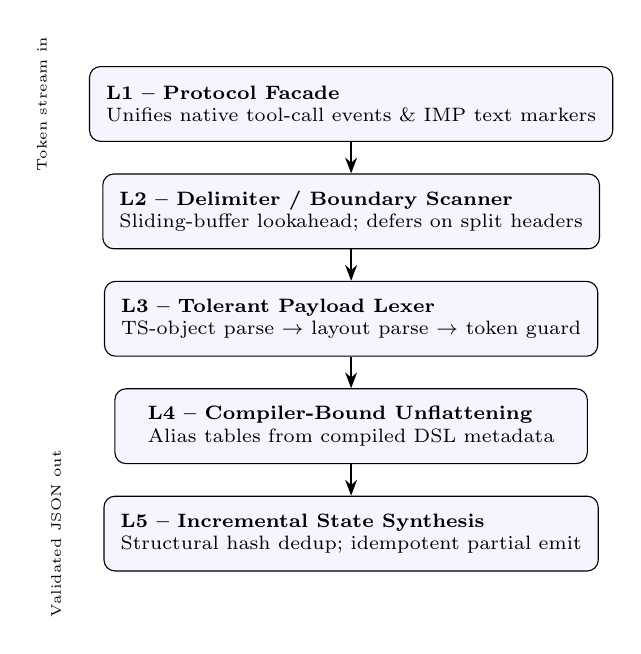
\begin{tikzpicture}[
  node distance=4mm,
  layer/.style={draw, rounded corners, minimum width=6.0cm,
                minimum height=0.95cm, align=left, font=\scriptsize,
                fill=blue!4, inner xsep=6pt},
  arr/.style={-{Stealth[length=2mm]}, thick}
]
\node[layer] (l1) {\textbf{L1 -- Protocol Facade}\\Unifies native tool-call events \& IMP text markers};
\node[layer, below=of l1] (l2) {\textbf{L2 -- Delimiter / Boundary Scanner}\\Sliding-buffer lookahead; defers on split headers};
\node[layer, below=of l2] (l3) {\textbf{L3 -- Tolerant Payload Lexer}\\TS-object parse $\to$ layout parse $\to$ token guard};
\node[layer, below=of l3] (l4) {\textbf{L4 -- Compiler-Bound Unflattening}\\Alias tables from compiled DSL metadata};
\node[layer, below=of l4] (l5) {\textbf{L5 -- Incremental State Synthesis}\\Structural hash dedup; idempotent partial emit};

\foreach \a/\b in {l1/l2, l2/l3, l3/l4, l4/l5}
  \draw[arr] (\a) -- (\b);

\node[left=6mm of l1, font=\tiny, rotate=90, anchor=center] {Token stream in};
\node[left=6mm of l5, font=\tiny, rotate=90, anchor=center] {Validated JSON out};
\end{tikzpicture}%
}
\caption{The five-layer IMP parser pipeline. Each layer's failure mode
and recovery strategy are detailed in Section~IV and traced to prior
architectural precedent in Section~II.}
\label{fig:architecture}
\end{figure}

\subsection{Layer 1: Dual-Mode Protocol Facade}
Unifies provider-native function-call events and IMP text markers into a
single Intent representation (\texttt{tool\_call}, \texttt{workflow\_call},
\texttt{helper\_call}, \texttt{response\_schema}), so downstream layers and
host application code are agnostic to execution mode.

\subsection{Layer 2: Stream Delimiter and Token Boundary Scanner}
Addresses \emph{token boundary tearing}: streaming transports deliver text
in arbitrary fragments, and a control delimiter such as
\texttt{[tool\_call:search]} may be split across packets. The scanner
maintains a sliding buffer and a set of known header prefixes; on a
prefix split at a chunk boundary, it defers extraction until the next
chunk resolves it, preventing partial control syntax from leaking into
user-visible output. For a completed stream, a known opening header may
use its line ending as a missing \texttt{]} boundary; incremental scans
remain strict so fragmented headers are not closed prematurely. This is a
direct application of the
resynchronization principle in \cite{burkefisher}, adapted from
statement-level tokens to protocol-level delimiters.

\subsection{Layer 3: Dual-Dialect Tolerant Payload Lexer}
Standard JSON parsers fail atomically on a single malformed token. The
lexer instead applies a fallback cascade: (1) a TypeScript-object-literal
parser accepting unquoted keys, single-quoted strings, and bare literals;
(2) an indentation-sensitive layout parser (in the lineage of
\cite{yamlspec}) for multi-line, brace-free key-value output; (3)
semantic token protection in the layout-parser path that guards
\texttt{@} and \texttt{.} inside string values from being misinterpreted
as structural delimiters. Bare single-line values containing \texttt{@}
are routed through this scalar-preserving path before brace-style parsing.

\subsection{Layer 4: Compiler-Bound Type Integration and Shape Unflattening}
The distinguishing contribution of this architecture: nested type
declarations in the IMP DSL are compiled into flat field specifications
and alias tables ahead of runtime, in the spirit of schema-compilation
systems such as \cite{protobuf,graphqlspec} but applied to
\emph{reconstruction} of non-conforming data rather than validation of
conforming data (Section~II-D). The parser consumes these
compiler-generated tables to reconstruct deeply nested objects from exact
underscore aliases (for example, \texttt{user\_address\_city}) and dotted
paths whose complete segment sequence is present in the same metadata.
Unknown dotted keys remain literal rather than being split heuristically.

\subsection{Layer 5: Incremental State Synthesis and Deduplicated Streaming}
Maintains a structural hash of the partial payload tree; identical
successive hashes (e.g., from whitespace-only deltas) suppress redundant
partial-state emission, preventing UI thrashing and duplicate
side-effects in host applications consuming live tool-argument previews.

\section{Fault Recovery Mechanics}

We define six malformed-stream patterns against which the architecture
in Section~III is evaluated, illustrated for the fragmentation case in
Fig.~\ref{fig:fragmentation}.

\textbf{Pattern 1 -- Syntax-corrupted payloads.} Unquoted keys, missing
commas, or brace-free layout text. Resolved by Layer 3's fallback cascade
without re-prompting.

\textbf{Pattern 2 -- Incomplete/truncated buffers.} A stream that
terminates mid-key-value (e.g., \texttt{age:} with no trailing value).
The line collector emits the fields resolved so far and assigns an
explicit null to the incomplete trailing field rather than raising a
deserialization exception.

\textbf{Pattern 3 -- Protocol-corrupted control delimiters.} Absent
\texttt{[/tool\_call]} tags are handled by implicit block termination at
end-of-stream or at the next recognized header. At finalization, a known
opening header missing \texttt{]} is recovered only when a line boundary
cleanly separates it from the payload.

\textbf{Pattern 4 -- Flat-to-nested structural mismatches.} Exact flat
aliases and schema-known dotted paths are reconstructed into nested objects
via Layer 4's alias tables; unknown dotted literals are preserved.

\textbf{Pattern 5 -- Transport-level fragmentation.} Delimiters and
payload text arbitrarily split across network chunks. Resolved by the
combination of Layer 2's lookahead buffering and Layer 5's structural
hash deduplication, which are designed to make parsed output invariant to
chunk boundaries; Section~V measures this property experimentally.

\textbf{Pattern 6 -- Ambiguous duplicate fields.} Repeated keys are not
``repaired'' by selecting a value. Final executable blocks are rejected;
longest-valid-prefix recovery is restricted to non-final partial state.

\paragraph{Canonical envelope and bounded recovery.} The canonical core
envelope is
\[
\begin{aligned}
S &::= B^*, & B_k &::= O_k\,P\,C(k),\\
O_k &::= \texttt{[}k\texttt{]} \mid \texttt{[}k\texttt{:}N\texttt{]},
& k &\in \mathcal{K}_{\mathrm{IMP}},
\end{aligned}
\]
where $N$ is a target name or metadata, $P$ is payload text, and $C(k)$ is
the registered closing marker for intent kind $k$. Recovery maps malformed
input to this envelope only under four execution-safety invariants: a final
intent requires a recognized, boundary-resolved opening marker; its payload
must parse without duplicate keys; structural expansion must match an exact
compiler-authorized path; and non-final prefix recovery may update partial UI
state but cannot authorize execution. End-of-stream header repair additionally
requires a newline boundary. Inputs outside these predicates are rejected;
recovery coverage is claimed only for the six evaluated patterns, not for
arbitrary corruption.

\begin{figure}[t]
\centering
\resizebox{\columnwidth}{!}{%
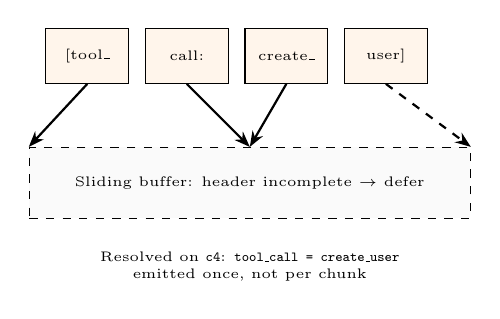
\begin{tikzpicture}[
  chunk/.style={draw, minimum width=1.05cm, minimum height=0.7cm,
                font=\tiny, fill=orange!8},
  buf/.style={draw, dashed, minimum width=5.6cm, minimum height=0.9cm,
              font=\tiny, fill=gray!4},
  node distance=2mm
]
\node[chunk] (c1) {[tool\_};
\node[chunk, right=of c1] (c2) {call:};
\node[chunk, right=of c2] (c3) {create\_};
\node[chunk, right=of c3] (c4) {user]};

\node[buf, below=8mm of c2, xshift=8mm] (buf) {Sliding buffer: header incomplete $\to$ defer};

\draw[-{Stealth[length=2mm]}, thick] (c1.south) -- (buf.north west);
\draw[-{Stealth[length=2mm]}, thick] (c2.south) -- (buf.north);
\draw[-{Stealth[length=2mm]}, thick] (c3.south) -- (buf.north);
\draw[-{Stealth[length=2mm]}, thick, dashed] (c4.south) -- (buf.north east);

\node[below=3mm of buf, font=\tiny, align=center]
  {Resolved on \texttt{c4}: \texttt{tool\_call = create\_user}\\emitted once, not per chunk};
\end{tikzpicture}%
}
\caption{Pattern 5: a single delimiter fragmented across four network
chunks is buffered by Layer 2 and resolved atomically once the header
closes; Layer 5's hash dedup prevents redundant emission on intermediate
chunks.}
\label{fig:fragmentation}
\end{figure}

\section{Experimental Methodology}

\subsection{Test Suites}

The corpus is fault-directed and stratified by parser transformation. Case
quotas are chosen to isolate recovery mechanisms and exact semantic outcomes,
not to approximate the prevalence of faults in deployed LLM traffic.
The 900-case corpus contains 750 recoverable cases with exact-AST oracles
(Suites A--C and the positive portion of Suite H) and 150 ambiguity controls
with rejection oracles (Suite E and the remaining portion of Suite H).

\textbf{Suite A -- Synthetic Syntax Corruption.} 100 unquoted-key/string
payloads; 100 indentation-only (brace-free) payloads; 100 comma-omission
payloads; and 50 special-character-protection payloads divided among
\texttt{@}, \texttt{.}, \texttt{:}, and \texttt{-} inside string values.

\textbf{Suite B -- Protocol and Boundary Corruption.} 50 unclosed-header
cases and 50 missing-closing-tag cases contribute to SRR. Separately, 100
valid streams are sliced at four chunk granularities (1 character, 5
characters, seeded-random boundaries, and monolithic baseline) and run 10
times each, producing 4,000 transport trials.

\textbf{Suite C -- Structural and Unflattening.} 100 dot-notation payloads
across 1--5 nesting levels; 50 key-alias payloads.

\textbf{Relation to prior real-model evaluation.} The preceding study tested
IMP with Qwen-3-32B, Llama-3.3-70B, and gpt-oss-120b \cite{irai2026}. The
present ablation freezes generation to isolate parser-layer effects. The prior
study supplies end-to-end evidence for its tested models; this study supplies
mechanism-level evidence but no new model-scale result or estimate of corruption
prevalence. The artifact can import provenance-labeled JSONL generations, but
SRR here denotes conditional recovery coverage.

\textbf{Baselines.} Config A removes only an exact protocol envelope and
uses strict JSON deserialization. A payload-only \texttt{json-repair}
v0.62.0 comparison is also run on Suites A and C. Because it does not
process the protocol envelope, it is reported separately rather than
inserted into the layer-wise ablation.
Generation-layer constrained decoding is not an additional ablation
configuration because it changes the upstream token distribution instead of
holding parser input constant; including it here would confound generator and
parser effects. A head-to-head comparison therefore requires a separate
end-to-end experiment with matched models, schemas, and latency boundaries.

\textbf{Suite E -- Over-Tolerance / False-Positive Suite.} 100 valid-JSON
objects containing conflicting duplicate keys. Rejection is the desired
outcome because silently selecting either value discards information.

\textbf{Suite H -- Template-Disjoint Regression Suite.} 200 cases generated from
templates and values distinct from the motivating suites: 50 single-line
unquoted emails, 50 unclosed headers with spacing and line-ending variants,
50 schema-known dotted paths at 2--5 levels, and 50 duplicate-key controls
across strict-JSON, brace-tolerant, and layout forms. The first 150 cases
contribute to SRR; the final 50 contribute to over-tolerance measurement.
The artifact records the immutable base revision and SHA-256 of the applied
parser-hardening patch.
Failures in the motivating suites and an initial regression pass informed the
hardening work. The patch was then frozen, and the complete 900-case corpus and
transport sweep were rerun from scratch.
The frozen source patch, generators, raw trials, analysis scripts, and checksum
manifest are available in an immutable repository snapshot \cite{artifact}.

Table~\ref{tab:cases} exposes representative corpus rows rather than only
aggregate counts. Each positive oracle is an exact semantic AST; rejection
is itself the oracle for an ambiguous duplicate.

\begin{table}[h]
\centering
\caption{Representative benchmark cases and their exact expected decisions.}
\label{tab:cases}
\scriptsize
\resizebox{\columnwidth}{!}{%
\begin{tabular}{@{}llll@{}}
\toprule
Fault & Representative payload & Oracle / decision & Layer \\
\midrule
Bare email & \texttt{contact: a+b@x.co} & \texttt{contact = "a+b@x.co"} & L3 \\
Unclosed header & \texttt{[tool\_call:bench\textbackslash n q:x} & \texttt{tool(bench, q=x)} & L2 \\
Missing tail tag & \texttt{[tool\_call:bench] q:x} & \texttt{tool(bench, q=x)} & L2 \\
Dotted path & \texttt{user.address.city: T} & \texttt{user.address.city = "T"} & L4 \\
Compiler alias & \texttt{user\_address\_city: T} & \texttt{user.address.city = "T"} & L4 \\
Duplicate key & \texttt{q:a\textbackslash n q:b} & Reject completed block & L3/L5 \\
\bottomrule
\end{tabular}}
\end{table}

\subsection{Metrics}

\begin{itemize}
\item \textbf{Syntactic Recovery Rate (SRR):} parsed ASTs exactly equal to
the case oracle / recoverable invocation attempts. Parser acceptance alone
does not count as recovery.
\item \textbf{Parser Time to First Partial State (TTFPS):} local elapsed time from supplying the first
chunk to the first valid partial-intent callback. This excludes generation,
network, rendering, and tool-execution latency.
\item \textbf{Transport Invariance Score:} \% identical parsed AST output
between monolithic and 1-character-fragmented delivery of the same
stream.
\item \textbf{Over-Tolerance Rate (new):} \% of all 150 ambiguity controls silently
accepted as a specific structure rather than flagged as ambiguous.
\end{itemize}

\subsection{Ablation Design}

\begin{table}[h]
\centering
\caption{Layer-Wise Ablation over 750 Recoverable Cases}
\begin{tabular}{@{}lll@{}}
\toprule
Config & Modules Included & SRR (\%) \\
\midrule
A -- Baseline & Exact envelope + strict JSON & 0.00 \\
B -- Stream Scanner & Layer 2 + strict JSON & 20.00 \\
C -- + Tolerant Lexer & B + Layer 3 & 76.00 \\
D -- Full System & C + Layer 4 & 100.00 \\
\bottomrule
\end{tabular}
\end{table}

Each case was run 10 times. SRR was identical across repetitions
(standard deviation 0.00 percentage points), as expected for deterministic
parser inputs. Timing distributions are reported over individual trials;
repeating deterministic correctness cases should not be interpreted as
independent evidence about LLM generation variability.

\section{Results}

Figure~\ref{fig:ablation} shows the principal ablation. The final-stream
scanner recovers both protocol-corruption families, raising SRR from
0.00\% to 20.00\% across the combined positive corpus. Adding the tolerant
lexer raises exact SRR to 76.00\%. Compiler-bound alias and dotted-path
unflattening contributes a further 24.00 percentage points, reaching
100.00\% for the full system.

\begin{figure}[t]
\centering
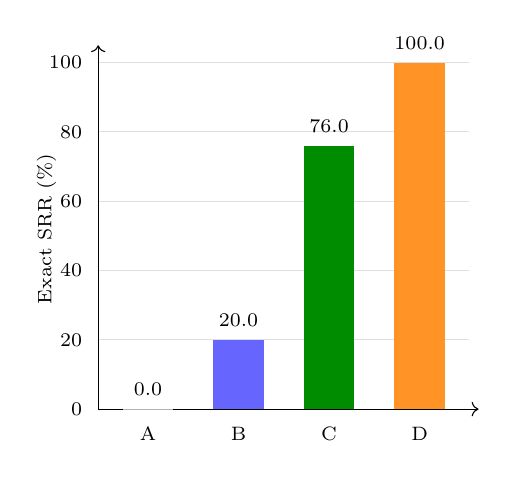
\begin{tikzpicture}[x=1.15cm,y=0.044cm,font=\scriptsize]
  \foreach \y in {0,20,40,60,80,100} {
    \draw[gray!25] (0.55,\y) -- (4.65,\y);
    \node[anchor=east] at (0.48,\y) {\y};
  }
  \draw[->] (0.55,0) -- (4.75,0);
  \draw[->] (0.55,0) -- (0.55,105);
  \node[rotate=90] at (-0.02,52) {Exact SRR (\%)};

  \fill[gray!60]        (0.82,0) rectangle (1.38,0.15);
  \fill[blue!60]        (1.82,0) rectangle (2.38,20.00);
  \fill[green!55!black] (2.82,0) rectangle (3.38,76.00);
  \fill[orange!85]      (3.82,0) rectangle (4.38,100.00);

  \foreach \x/\label in {1.10/A,2.10/B,3.10/C,4.10/D}
    \node[anchor=north] at (\x,-2.5) {\label};
  \node[anchor=south] at (1.10,1.2) {0.0};
  \node[anchor=south] at (2.10,21.0) {20.0};
  \node[anchor=south] at (3.10,77.0) {76.0};
  \node[anchor=south] at (4.10,101.0) {100.0};
\end{tikzpicture}
\caption{Exact syntactic recovery over 750 positive cases. Error bars are
zero because all 10 deterministic repetitions produced identical
correctness outcomes.}
\label{fig:ablation}
\end{figure}

\begin{table}[h]
\centering
\caption{Exact SRR by Test Suite (\%)}
\begin{tabular}{@{}lrrrr@{}}
\toprule
Configuration & Syntax A & Protocol B & Structure C & Regression H \\
\midrule
A -- Strict JSON & 0.00 & 0.00 & 0.00 & 0.00 \\
B -- Scanner & 0.00 & 100.00 & 0.00 & 33.33 \\
C -- Tolerant lexer & 100.00 & 100.00 & 13.33 & 66.67 \\
D -- Full system & 100.00 & 100.00 & 100.00 & 100.00 \\
\bottomrule
\end{tabular}
\end{table}

The full system recovered every syntax, protocol, structural, and positive
regression case. End-of-stream header repair is conservative: it uses a line
ending as the missing \texttt{]} boundary only for a completed stream, so
incremental scans do not prematurely close a fragmented header. Dotted
paths are reconstructed only when the complete path occurs in compiler
schema metadata; unknown dotted literals remain flat. Single-line emails
are routed through the layout scalar parser, preserving \texttt{@}, dots,
plus signs, and hyphens.

Across the transport sweep, final ASTs under one-character fragmentation
were identical to monolithic delivery in 100.00\% of trials. On the test
machine, one-character parser TTFPS had a 0.3080~ms median and 0.5281~ms
95th percentile. These values measure local parser work only and are not
comparable to end-to-end constrained-decoding or provider API latency.

\begin{figure}[t]
\centering
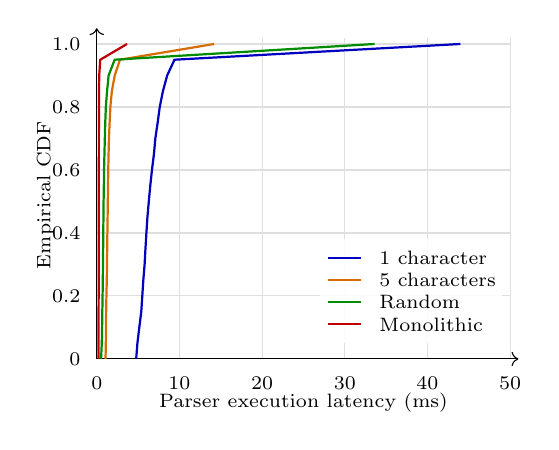
\begin{tikzpicture}[x=0.105cm,y=4.0cm,font=\scriptsize]
  \foreach \x in {0,10,20,30,40,50} {
    \draw[gray!25] (\x,0) -- (\x,1.02);
    \node[anchor=north] at (\x,-0.025) {\x};
  }
  \foreach \y in {0,0.2,0.4,0.6,0.8,1.0} {
    \draw[gray!25] (0,\y) -- (50,\y);
    \node[anchor=east] at (-0.8,\y) {\y};
  }
  \draw[->] (0,0) -- (51,0);
  \draw[->] (0,0) -- (0,1.05);
  \node at (25,-0.14) {Parser execution latency (ms)};
  \node[rotate=90] at (-6.2,0.52) {Empirical CDF};

  \draw[blue!75!black,thick] plot coordinates {
    (4.768,0.00) (4.916,0.05) (5.145,0.10) (5.384,0.15)
    (5.508,0.20) (5.631,0.25) (5.786,0.30) (5.889,0.35)
    (6.004,0.40) (6.127,0.45) (6.294,0.50) (6.472,0.55)
    (6.676,0.60) (6.914,0.65) (7.086,0.70) (7.364,0.75)
    (7.617,0.80) (8.002,0.85) (8.517,0.90) (9.400,0.95)
    (43.990,1.00)
  };
  \draw[orange!85!black,thick] plot coordinates {
    (1.060,0.00) (1.098,0.05) (1.116,0.10) (1.134,0.15)
    (1.168,0.20) (1.214,0.25) (1.235,0.30) (1.260,0.35)
    (1.284,0.40) (1.312,0.45) (1.336,0.50) (1.364,0.55)
    (1.390,0.60) (1.428,0.65) (1.473,0.70) (1.554,0.75)
    (1.648,0.80) (1.823,0.85) (2.172,0.90) (2.807,0.95)
    (14.198,1.00)
  };
  \draw[green!55!black,thick] plot coordinates {
    (0.519,0.00) (0.609,0.05) (0.646,0.10) (0.671,0.15)
    (0.703,0.20) (0.732,0.25) (0.746,0.30) (0.771,0.35)
    (0.786,0.40) (0.808,0.45) (0.826,0.50) (0.857,0.55)
    (0.880,0.60) (0.928,0.65) (0.975,0.70) (1.027,0.75)
    (1.099,0.80) (1.245,0.85) (1.433,0.90) (2.162,0.95)
    (33.609,1.00)
  };
  \draw[red!75!black,thick] plot coordinates {
    (0.211,0.00) (0.216,0.05) (0.218,0.10) (0.220,0.15)
    (0.229,0.20) (0.233,0.25) (0.235,0.30) (0.236,0.35)
    (0.238,0.40) (0.240,0.45) (0.243,0.50) (0.246,0.55)
    (0.249,0.60) (0.254,0.65) (0.256,0.70) (0.259,0.75)
    (0.263,0.80) (0.272,0.85) (0.296,0.90) (0.419,0.95)
    (3.664,1.00)
  };

  \begin{scope}[shift={(28,0.08)}]
    \fill[white,opacity=0.88] (-1,-0.03) rectangle (21,0.30);
    \draw[blue!75!black,thick] (0,0.24) -- (4,0.24);
    \node[anchor=west] at (5,0.24) {1 character};
    \draw[orange!85!black,thick] (0,0.17) -- (4,0.17);
    \node[anchor=west] at (5,0.17) {5 characters};
    \draw[green!55!black,thick] (0,0.10) -- (4,0.10);
    \node[anchor=west] at (5,0.10) {Random};
    \draw[red!75!black,thick] (0,0.03) -- (4,0.03);
    \node[anchor=west] at (5,0.03) {Monolithic};
  \end{scope}
\end{tikzpicture}
\caption{Empirical CDF of local parser execution time under four transport
chunking modes. This is a parser-fragmentation comparison, not an
end-to-end comparison with constrained decoding.}
\label{fig:transport-cdf}
\end{figure}

The payload-only \texttt{json-repair} baseline achieved 20.00\% exact SRR
on Suites A and C. Its exact recoveries were confined to the 100
unquoted-key/string cases; it did not exactly recover the layout,
comma-omission, protected-scalar, alias, or dotted-path categories. Because it
does not interpret IMP envelopes, its transport latency is not compared with
the full IMP parser. On the 150 conflicting duplicate-key controls, strict
JSON and scanner-plus-JSON each had a 75.33\% over-tolerance rate. Both
tolerant-lexer configurations rejected every control, yielding 0.00\%
over-tolerance. The remaining strict-baseline acceptances reflect duplicate
selection by the JSON deserializer rather than safe disambiguation.

\section{Discussion and Threats to Validity}

\textbf{Construct validity.} The evaluation measures deterministic parser
recovery, not end-to-end agent reliability or the model's latent intent. Its
synthetic generators cover named corruption families but are not a probability
sample of deployed LLM failures; SRR is therefore conditional corpus coverage,
not a forecast of deployment-wide success. \textbf{Internal validity.} Exact
oracles and deterministic inputs make configurations reproducible but do not
sample generator variance. The template-disjoint regression suite, frozen
patch, and artifact checksums limit implementation drift, but not benchmark
designer bias. \textbf{External validity.} Real-model compatibility and token
scaling across Qwen-3-32B, Llama-3.3-70B, and gpt-oss-120b were evaluated in
\cite{irai2026}; they are not re-run here because generation is held constant
to isolate parser layers. This paper therefore adds no new model-family
generalization, BFCL/ToolBench accuracy, or true first-pass execution claim.
Prompt-token reduction is inherited from \cite{irai2026}, and no
generation-layer constrained-decoder or provider-native latency baseline was
executed.

The results support bounded recovery rather than unrestricted repair.
Unclosed headers are repaired only at end-of-stream and only when a line
boundary separates header from payload. Dotted keys are unflattened only
when the path is authorized by compiler metadata, preventing accidental
reinterpretation of literal keys such as metric names. Duplicate detection
rejects the whole completed block; prefix recovery remains available only
for non-executable partial UI state. These policies improve coverage while
retaining an explicit ambiguity boundary.

\section{Conclusion}

This work opens the parser previously treated as a black box in
\cite{irai2026} and quantifies the contribution and limits of its layers.
On 750 recoverable synthetic cases, tolerant lexical parsing delivered the
largest increase, while compiler-bound structural unflattening added 24.00
percentage points for a 100.00\% full-system exact SRR. Streaming delivery
was invariant even at one character per chunk, and the full system rejected
all 150 duplicate-key controls. These results support downstream tolerant parsing as a
useful, model-agnostic recovery layer with bounded, schema-aware repair. The
real-model evidence remains that of the preceding study; a direct comparison
with generation-layer constrained decoding and broader model families remains
future work rather than a claim of this ablation.

\begin{thebibliography}{00}
\bibitem{irai2026} A. T. Junior and A. N. Baidoo, ``Decoupling Schema
Validation in Large Language Models: A Comparative Analysis of Intent
Marker Parsers vs. Traditional JSON Function Calling,'' \emph{IRAI 2026},
in press.
\bibitem{xgrammar} T. Dong et al., ``XGrammar: Flexible and efficient
structured generation engine for large language models,''
arXiv:2411.15100, 2024.
\bibitem{sglang} L. Zheng et al., ``SGLang: Efficient execution of
structured language model programs,'' \emph{NeurIPS}, vol. 37, 2024.
\bibitem{outlines} B. T. Willard and R. Louf, ``Efficient guided
generation for large language models,'' arXiv:2307.09702, 2023.
\bibitem{instructor} J. Liu, ``Instructor: Structured outputs for LLMs,''
GitHub repository, 2023.
\bibitem{bfcl} S. G. Patil et al., ``The Berkeley Function Calling
Leaderboard,'' \emph{ICML}, 2025.
\bibitem{jsonschemabench} S. Geng et al., ``JSONSchemaBench: Evaluating
constrained decoding with LLMs,'' ES-FoMo III Workshop, NeurIPS, 2024.
\bibitem{burkefisher} M. Burke and G. A. Fisher, ``A practical method for
LR and LL syntactic error diagnosis and recovery,'' \emph{ACM
Transactions on Programming Languages and Systems (TOPLAS)}, vol. 9,
no. 2, pp. 164--197, 1987, doi: 10.1145/22719.22720.
\bibitem{wagnergraham} T. A. Wagner and S. L. Graham, ``Efficient and
flexible incremental parsing,'' \emph{ACM TOPLAS}, vol. 20, no. 5,
pp. 980--1013, 1998, doi: 10.1145/293677.293678.
\bibitem{treesitter} M. Brunsfeld et al., ``tree-sitter: An incremental
parsing system for programming tools,'' software repository. [Online].
Available: \url{https://github.com/tree-sitter/tree-sitter}
\bibitem{yamlspec} O. Ben-Kiki, C. Evans, and I. d\"ot Net, ``YAML Ain't
Markup Language (YAML) Version 1.1,'' final draft, Jan. 2005. [Online].
Available: \url{https://yaml.org/spec/1.1/}
\bibitem{json5spec} A. Kishore and J. Tucker, ``The JSON5 Data Interchange
Format,'' 2017. [Online]. Available: \url{https://spec.json5.org/}
\bibitem{protobuf} Google, ``Protocol Buffers Programming Guides.''
[Online]. Available: \url{https://protobuf.dev/programming-guides/}
\bibitem{graphqlspec} GraphQL Foundation, ``GraphQL Specification,''
Oct. 2021. [Online]. Available: \url{https://spec.graphql.org/October2021/}
\bibitem{baml-sap} V. Gupta, ``Prompting vs JSON Mode vs Function Calling
vs Constrained Generation vs SAP,'' BoundaryML. [Online]. Available:
\url{https://boundaryml.com/blog/schema-aligned-parsing}. [Accessed: Aug. 8, 2026].
\bibitem{baml-docs} BoundaryML, ``Why BAML?'' BAML Documentation. [Online].
Available: \url{https://docs.boundaryml.com/guide/introduction/why-baml}.
[Accessed: Aug. 8, 2026].
\bibitem{artifact} A. T. Junior, E. M. Martey, D. M. Gyielzaw, and
A. M. A. Dwamena, ``Auwgent intent-parser ablation artifact,'' GitHub
repository, commit dcecb84eac086f46c9e39d745eb21fdd5b58f145, 2026.
[Online]. Available:
\url{https://github.com/snrraptopack/Auwgent/tree/dcecb84eac086f46c9e39d745eb21fdd5b58f145/benchmarks/intent-parser-paper}
\bibitem{jsonrepair} S. Baccianella, ``JSON Repair---A Python module to
repair invalid JSON, commonly used to parse the output of LLMs,'' software,
2025. [Online]. Available: \url{https://github.com/mangiucugna/json_repair}
\end{thebibliography}

\end{document}
